\subsection{Experimentación}

En esta sección se presentan los experimentos realizados para evaluar el rendimiento del algoritmo Q-Learning en el entorno. Se analiza cómo diferentes parámetros del algoritmo afectan su capacidad para encontrar políticas óptimas, su convergencia y su eficiencia.

\subsubsection{Experimento factor de descuento \& tasa de aprendizaje}

\paragraph{Diseño experimental}

El objetivo de este experimento es analizar cómo el factor de descuento y la tasa de aprendizaje afectan el rendimiento del algoritmo Q-Learning.

% TODO: Usar esta tabla para cada experimento
\begin{table}[H]
    \centering
    \begin{tabularx}{\textwidth}{|p{4cm}|X|} % Especificar el ancho de las columnas
        \hline % Línea horizontal superior
        \textbf{Observación} & El factor de descuento ($\gamma$) y la tasa de aprendizaje ($\alpha$) de exploración son parámetros críticos en el algoritmo Q-Learning. 
        \\ \hline 
        \textbf{Planteamiento} & Para cada pareja de valores de $\gamma$ y $\alpha$, se compara la tasa de acierto (llegar al estado final), la recompensa media, número de pasos y tiempo de entrenamiento del algoritmo.
        \\ \hline 
        \textbf{Hipótesis} & Un mayor factor de descuento y una tasa de aprendizaje más lenta mejorarán el rendimiento del algoritmo.
        \\ \hline 
        \textbf{Método} & 
        \begin{itemize}
            \item Se fijan 1000 episodios de entrenamiento, \(\epsilon\) inicial de $0.9$, coeficiente de decaimiento de \(\epsilon\) de $0.95$, un coeficiente de decaimiento de la tasa de aprendizaje de $0.99$ y una penalización de la acción ``moverse a la izquierda'' de $-1$.
            \item Se eligen los siguientes valores para \(\gamma\) y $\alpha$: \(\gamma \in \{0.5, 0.7, 0.9, 0.95, 0.99\}\) y $\alpha \in \{0.1, 0.2, 0.5, 0.8\}$.
            \item Para cada combinación de \(\gamma\) y $\alpha$, se ejecuta el algoritmo Q-Learning en el entorno.
            \item Se evalúa la política obtenida probándola con 500 episodios.
            \item Se repite el proceso para cada combinación de \(\gamma\) y $decay$ 20 veces para obtener una muestra representativa (debido a la estocasticidad del entorno).
        \end{itemize}
        \\ \hline
    \end{tabularx}
    \caption{Q-Learning - Experimento 1 - Factor de descuento \& tasa de aprendizaje}
    \label{tab:diseñoQLEarningExp1}
\end{table}

\paragraph{Resultados}

Los resultados del experimento se han representado mediante heatmaps para facilitar la visualización de los datos. En cada gráfico, el eje X representa el factor de descuento ($\gamma$) y el eje Y representa la tasa de aprendizaje ($\alpha$). Los colores indican el valor de la métrica correspondiente. Cada valor representa la media de las 20 ejecuciones del algoritmo (cada ejecución está representada por la media de 500 episodios) de la correspondiente combinación de parámetros. 
\\

\textbf{Tasa de Éxito}

\begin{figure}[H]
    \centering
    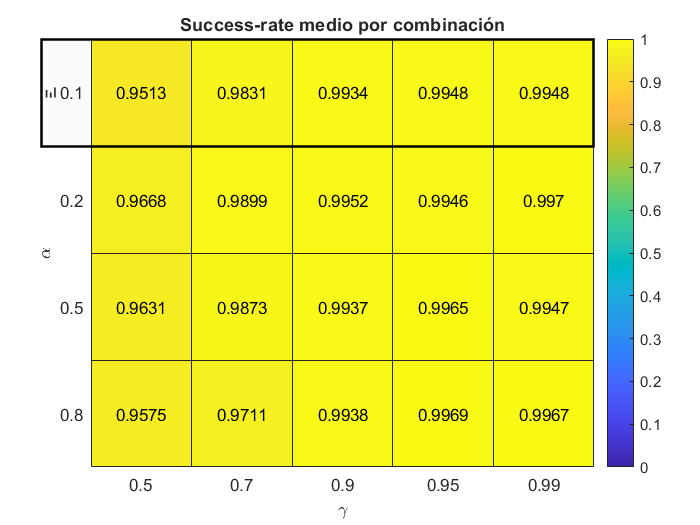
\includegraphics[width=0.7\textwidth]{../../experiments/qlearning/experiment-1/results/success.png}
    \caption{Tasa de éxito para diferentes combinaciones de $\alpha$ y $\gamma$}
    \label{fig:qlearning-success}
\end{figure}

En general, la tasa de éxito en este caso es bastante alta para todas las combinaciones de valores. Sin embargo, puede observarse una pequeña tendencia. Conforme aumenta el factor de descuento ($\gamma$), el porcentaje de éxito se aproxima a 1. 

\begin{itemize}
    \item Con $\gamma = 0.5$, la tasa de éxito se mantiene alrededor del 95-96\%
    \item Para $\gamma \geq 0.9$, la tasa de éxito supera consistentemente el 99\%
\end{itemize}

La mejor combinación se alcanza con $\gamma = 0.99$ y $\alpha = 0.2$, logrando una tasa de éxito del 99.7\%

\newpage

\textbf{Recompensa media y número de pasos medios}

\begin{figure}[H]
    \centering
    \begin{subfigure}{0.7\textwidth}
        \centering
        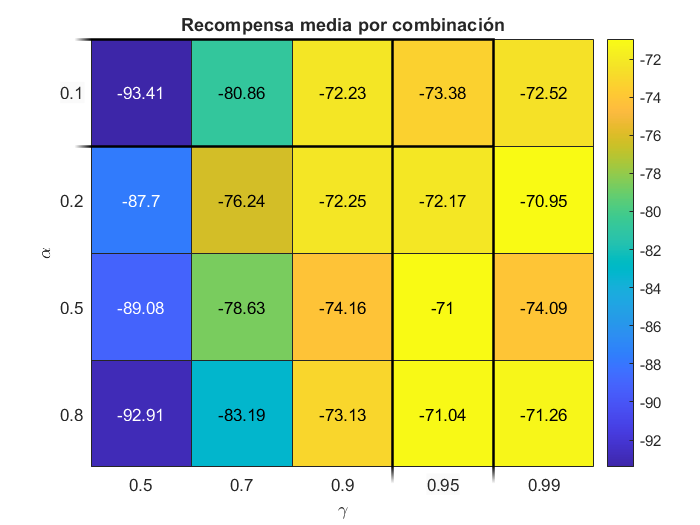
\includegraphics[width=\textwidth]{../../experiments/qlearning/experiment-1/results/reward.png}
        \caption{Recompensa media para diferentes combinaciones de $\alpha$ y $\gamma$}
        \label{fig:qlearning-subfig-reward}
    \end{subfigure}
    \hfill
    \begin{subfigure}{0.7\textwidth}
        \centering
        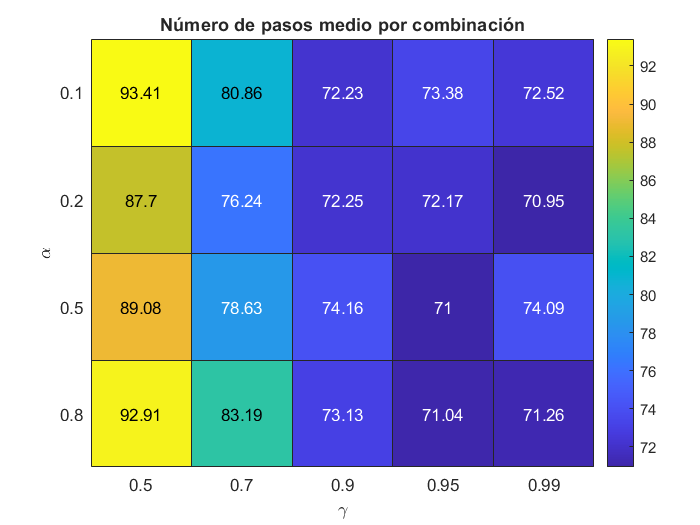
\includegraphics[width=\textwidth]{../../experiments/qlearning/experiment-1/results/steps.png}
        \caption{Número de pasos para diferentes combinaciones de $\alpha$ y $\gamma$}
        \label{fig:qlearning-subfig-steps}
    \end{subfigure}
    \caption{Análisis de la recompensa media y número de pasos}
    \label{fig:qlearning-reward}
\end{figure}

El análisis de la recompensa media y el número medio de pasos revela que:

\begin{itemize}
    \item Las recompensas mejoran significativamente (son menos negativas) al aumentar $\gamma$ y, por lo tanto, el número de pasos también se reduce. 
    \item La tasa de aprendizaje no tiene mucha influencia en esta cambinación de parámetros. 
    \item Con $\gamma = 0.5$, las recompensas medias oscilan entre -93 y -87, representando trayectorias más largas.
    \item Las mejores recompensas se obtienen con $\gamma \geq 0.9$, alcanzando valores cercanos a -70.
\end{itemize}

La combinación óptima es $\gamma = 0.99$, $\alpha = 0.2$ y logra una recompensa media de -70.95. Corresponde con la combinación que obtiene mejor tasa de éxito. 
\\

Se puede observar que el número medio de pasos corresponde exactamente con la recompensa media en cada configuración. Esto nos indica que el agente no cae por el barranco en ningún momento, ya que sino la recompensa media sería más negativa (-100 de recompensa por caer en 1 paso, perderia la correspondencia de -1 de recompensa por cada paso).
\\

\textbf{Tiempo de entrenamiento}
\\

Para el tiempo de entrenamiento, se han elegido las tres combinaciones que mejor rendimiento han dado. 

\begin{figure}[H]
    \centering
    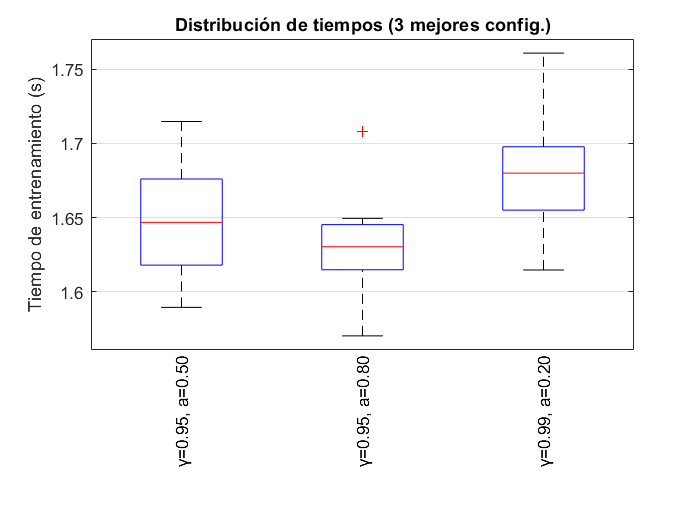
\includegraphics[width=0.8\textwidth]{../../experiments/qlearning/experiment-1/results/time.png}
    \caption{Tiempo de entrenamiento para diferentes combinaciones de $\alpha$ y $\gamma$}
    \label{fig:qlearning-time}
\end{figure}

El análisis del tiempo de ejecución muestra que para las tres combinaciones, el tiempo se mueve entorno a los 1.65 segundos. Hay poca diferencia entre ellos, con una pequeña variabilidad en las colas. 
\\

\newpage

\textbf{Tabla resumen}

\begin{table}[H]
    \centering
    \begin{tabular}{|c|c|l|r|c|}
    \hline
    $\gamma$ & $\alpha$ & Métrica        & Media    & Intervalo de Confianza del 95\% \\
    \hline
    0.95 & 0.50 & Success-rate  & 0.997   & [0.993, 1.000] \\
         &      & Rew. media    & -71.000 & [-74.340, -67.660] \\
         &      & Steps medios  & 71.0    & [67.7, 74.3] \\
         &      & Time (s)      & 1.65    & [1.62, 1.67] \\
    \hline
    0.95 & 0.80 & Success-rate  & 0.997   & [0.994, 1.000] \\
         &      & Rew. media    & -71.039 & [-73.977, -68.101] \\
         &      & Steps medios  & 71.0    & [68.1, 74.0] \\
         &      & Time (s)      & 1.63    & [1.61, 1.65] \\
    \hline
    0.99 & 0.20 & Success-rate  & 0.997   & [0.995, 0.999] \\
         &      & Rew. media    & -70.945 & [-73.840, -68.051] \\
         &      & Steps medios  & 70.9    & [68.1, 73.8] \\
         &      & Time (s)      & 1.68    & [1.66, 1.71] \\
    \hline
    \end{tabular}
    \caption{Resultados para combinaciones seleccionadas de $\gamma$ y $\alpha$}
    \label{tab:resultados_seleccionados}
    \end{table}

\textbf{Conclusiones}
\\

Del análisis experimental se pueden extraer las siguientes conclusiones:

\begin{enumerate}
    \item El factor de descuento ($\gamma$) tiene un impacto más significativo que la tasa de aprendizaje ($\alpha$) en el rendimiento del algoritmo con la configuración de parámetro definida.
    \item Los valores óptimos se encuentran en el rango de $\gamma \geq 0.9$.
    \item La tasa de aprendizaje óptima parece estar entre 0.2 y 0.5.
    \item La mejor combinación general considerando todas los métricas es $\gamma = \textbf{0.99}$ y $\alpha = \textbf{0.2}$, que proporciona:
    \begin{itemize}
        \item Una tasa de éxito del 99.7\%.
        \item Una recompensa media de -70.95.
        \item Un tiempo de entrenamiento de 1.68 segundos.
    \end{itemize}
    \item Los resultados obtenidos confirman la hipótesis inicial de que un mayor factor de descuento y una tasa de aprendizaje más lenta mejoran el rendimiento del algoritmo.
\end{enumerate}

Aunque los parámetros seleccionados no minimizan el tiempo de entrenamiento, las diferencias temporales observadas son mínimas. En este estudio se ha priorizado la optimización de la tasa de aciertos y la recompensa sobre el tiempo de entrenamiento, ya que estos criterios son más relevantes para evaluar la efectividad del algoritmo.

\newpage
\subsubsection{Experimento tasa de exploración (\(\epsilon\)) \& decaimiento de la tasa de exploración (\(\epsilon\))}

\paragraph{Diseño experimental}
El objetivo de este experimento es analizar cómo la tasa de exploración y su decaimiento afectan el rendimiento del algoritmo Q-Learning.

\begin{table}[H]
    \centering
    \begin{tabularx}{\textwidth}{|p{4cm}|X|} % Especificar el ancho de las columnas
        \hline % Línea horizontal superior
        \textbf{Observación} & El rendimiento y óptimalidad de la política encontrada por Q-Learning se ven afectados por la tasa de exploración y su decaimiento. 
        \\ \hline 
        \textbf{Planteamiento} & Para cada combinación de \(\epsilon\) y decaimiento de \(\epsilon\), se compara la tasa de acierto (llegar al estado final), la recompensa media, número de pasos y tiempo de entrenamiento del algoritmo.
        \\ \hline 
        \textbf{Hipótesis} & Un mayor valor de \(\epsilon\) y un decaimiento moderado mejorarán el rendimiento del algoritmo.
        \\ \hline 
        \textbf{Método} & 
        \begin{itemize}
            \item Se fijan 1000 episodios de entrenamiento,  un coeficiente de decaimiento de la tasa de aprendizaje de $0.99$, una penalización de la acción ``moverse a la izquierda'' de $-1$. y los mejores valores para \(\gamma\) y $\alpha$ del experimento anterior.
            \item Se eligen los siguientes valores para \(\epsilon\) y decaimiento de \(\epsilon\): \(\epsilon \in \{0.7, 0.9, 0.95, 0.99\}\) y decaimiento de \(\epsilon \in \{0.8, 0.9, 0.95, 0.99\}\).
            \item Para cada combinación de \(\epsilon\) y decaimiento de \(\epsilon\), se ejecuta el algoritmo Q-Learning en el entorno.
            \item Se evalúa la política obtenida probándola con 500 episodios.
            \item Se repite el proceso para cada combinación de \(\epsilon\) y decaimiento de \(\epsilon\) 20 veces para obtener una muestra representativa (debido a la estocasticidad del entorno).
        \end{itemize}
        \\ \hline
    \end{tabularx}
    \caption{Q-Learning - Experimento 2 - Tasa de exploracion \& decaimiento de la tasa de exploracion}
    \label{tab:diseñoQLEarningExp2}
\end{table}
\newpage
\paragraph{Resultados}

Los resultados del experimento se han representado mediante heatmaps para facilitar la visualización de los datos. En cada gráfico, el eje X representa la tasa de exploración ($\epsilon$) y el eje Y representa el decaimiento de la tasa de exploración. Los colores indican el valor de la métrica correspondiente. Cada valor representa la media de las 20 ejecuciones del algoritmo (cada ejecución está representada por la media de 500 episodios) de la correspondiente combinación de parámetros. 
\\

\textbf{Tasa de Éxito}

\begin{figure}[H]
    \centering
    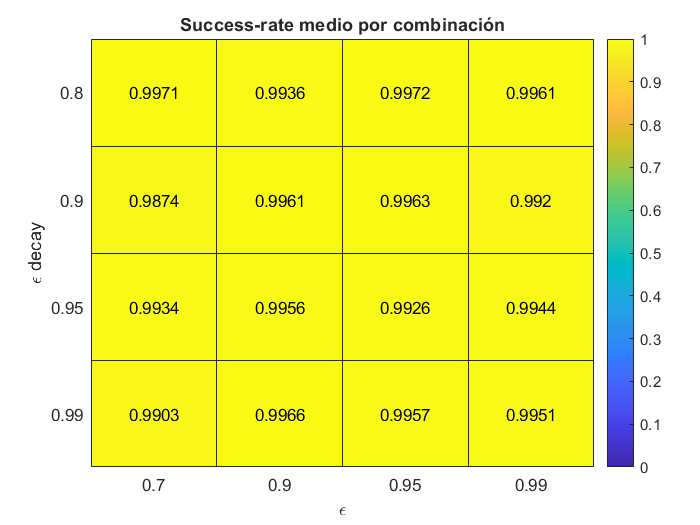
\includegraphics[width=0.7\textwidth]{../../experiments/qlearning/experiment-2/results/success.png}
    \caption{Tasa de éxito para diferentes combinaciones de $\epsilon$ y su decaimiento}
    \label{fig:qlearning-success}
\end{figure}
La tasa de éxito también es bastante elevada en este caso y no se observa ninguna tendencia clara. Todos los valores se encuentran entre el 98.7\% y el 99.7\%.

La mejor combinación se alcanza con $\epsilon = 0.95$ y su decaimiento = 0.8, logrando una tasa de éxito del 99.72\%.


\newpage

\textbf{Recompensa media y número de pasos medios}

\begin{figure}[H]
    \centering
    \begin{subfigure}{0.7\textwidth}
        \centering
        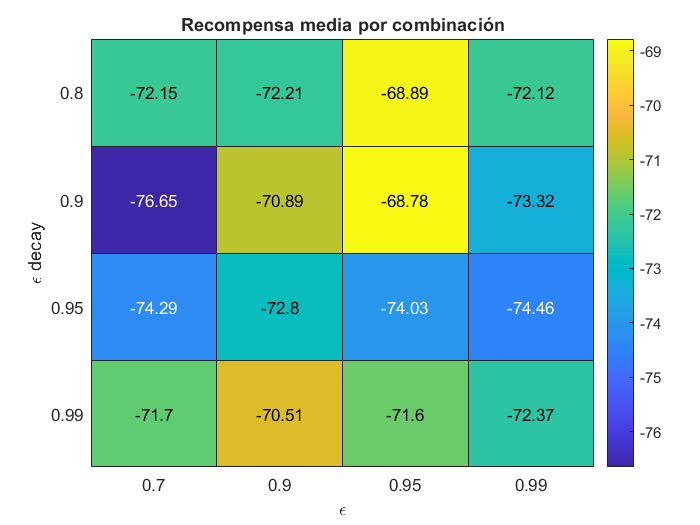
\includegraphics[width=\textwidth]{../../experiments/qlearning/experiment-2/results/reward.png}
        \caption{Recompensa media para diferentes combinaciones de $\epsilon$ y su decaimiento}
        \label{fig:qlearning-subfig-reward}
    \end{subfigure}
    \hfill
    \begin{subfigure}{0.7\textwidth}
        \centering
        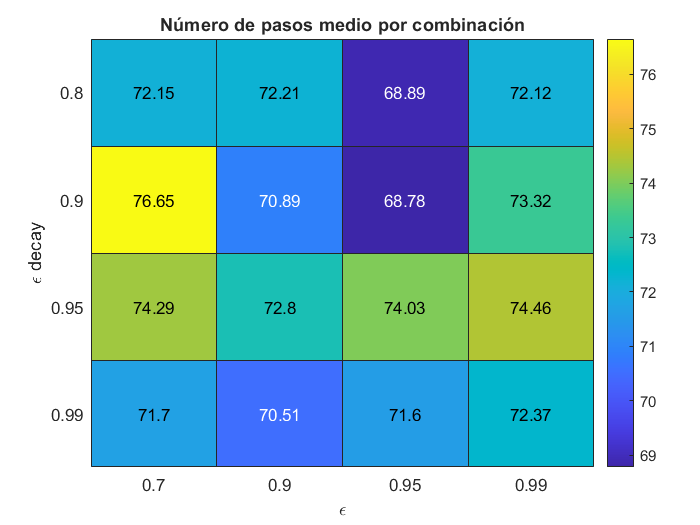
\includegraphics[width=\textwidth]{../../experiments/qlearning/experiment-2/results/steps.png}
        \caption{Número de pasos para diferentes combinaciones de $\epsilon$ y su decaimiento}
        \label{fig:qlearning-subfig-steps}
    \end{subfigure}
    \caption{Análisis de la recompensa media y número de pasos}
    \label{fig:qlearning-reward}
\end{figure}

El análisis de la recompensa media y el número medio de pasos tampoco revela una tendencia clara. Lo que si que se puede observar es que todas las configuraciones se encuentran entre -76.65 y -68.79 de recompensa, lo que indica que ninguna de ellas se desvia ni obtiene resultados muy negativos. 
\\

Se puede observar también que el número medio de pasos corresponde exactamente con la recompensa media en cada configuración. Esto nos indica que el agente no cae por el barranco en ningún momento, ya que sino la recompensa media sería más negativa.
\\

Las combinaciones óptimas son $\epsilon = 0.95$ y su decaimiento = 0.8, logrando una recompensa media de -68.89, y $\epsilon = 0.95$ y su decaimiento = 0.9, logrando una recompensa media de -68.78.
\\

\textbf{Tiempo de entrenamiento}
\\

Para el tiempo de entrenamiento, se han elegido las tres combinaciones que mejor rendimiento han dado. 

\begin{figure}[H]
    \centering
    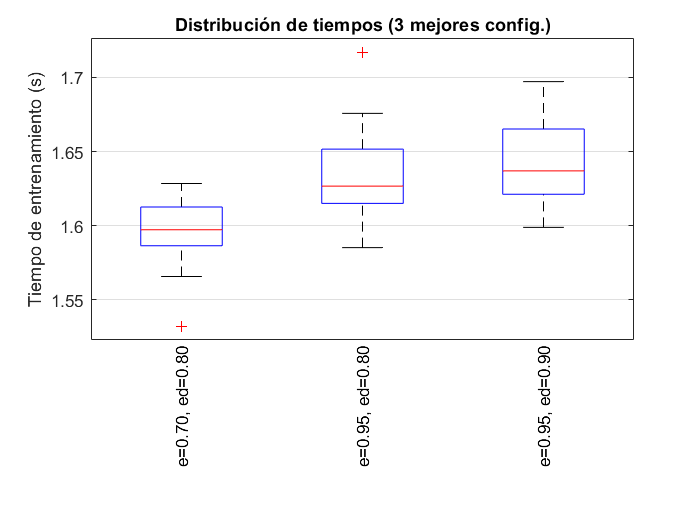
\includegraphics[width=0.8\textwidth]{../../experiments/qlearning/experiment-2/results/time.png}
    \caption{Tiempo de entrenamiento para diferentes combinaciones de $\epsilon$ y su decaimiento}
    \label{fig:qlearning-time}
\end{figure}

El análisis del tiempo de ejecución muestra que para las tres combinaciones, el tiempo se mueve entorno a los 1.62 segundos. Hay poca diferencia entre ellos, con una pequeña variabilidad en las colas. 
\\

\newpage
\textbf{Tabla resumen}

\begin{table}[H]
    \centering
    \begin{tabular}{|c|c|l|r|c|}
    \hline
    $\epsilon$ & $decay$ & Métrica        & Media    & Intervalo de Confianza del 95\% \\
    \hline
    0.70 & 0.80 & Success-rate  & 0.997   & [0.995, 0.999] \\
         &      & Rew. media    & -72.150 & [-75.391, -68.910] \\
         &      & Steps medios  & 72.2    & [68.9, 75.4] \\
         &      & Time (s)      & 1.60    & [1.58, 1.61] \\
    \hline
    0.95 & 0.80 & Success-rate  & 0.997   & [0.995, 0.999] \\
         &      & Rew. media    & -68.889 & [-70.869, -66.909] \\
         &      & Steps medios  & 68.9    & [66.9, 70.9] \\
         &      & Time (s)      & 1.63    & [1.61, 1.66] \\
    \hline
    0.95 & 0.90 & Success-rate  & 0.996   & [0.990, 1.003] \\
         &      & Rew. media    & -68.782 & [-72.091, -65.473] \\
         &      & Steps medios  & 68.8    & [65.5, 72.1] \\
         &      & Time (s)      & 1.64    & [1.62, 1.66] \\
    \hline
    \end{tabular}
    \caption{Resultados para combinaciones seleccionadas de $\epsilon$ y $decay$}
    \label{tab:resultados_seleccionados}
\end{table}
    
    

\textbf{Conclusiones}
\\

Del análisis experimental se pueden extraer las siguientes conclusiones:

\begin{enumerate}
    \item La tasa de exploración y su decaimiento no parecen tener un impacto significativo en el rendimiento del algoritmo Q-Learning.
    \item La mejor combinación general considerando todas los métricas es $\epsilon = \textbf{0.95}$ y su decaimiento = \textbf{0.8}, que proporciona:
    \begin{itemize}
        \item Una tasa de éxito del 99.72\%.
        \item Una recompensa media de -68.89.
        \item Un tiempo de entrenamiento de 1.63 segundos.
    \end{itemize}
    \item Los resultados obtenidos confirman la hipótesis inicial de que un mayor valor de \(\epsilon\) y un decaimiento moderado mejoran el rendimiento del algoritmo. 
\end{enumerate}

Aunque los parámetros seleccionados no minimizan el tiempo de entrenamiento, las diferencias temporales observadas son mínimas. En este estudio se ha priorizado la optimización de la tasa de aciertos y la recompensa sobre el tiempo de entrenamiento, ya que estos criterios son más relevantes para evaluar la efectividad del algoritmo.

\newpage
\subsubsection{Experimento tasa de aprendizaje \& decaimiento de la tasa de aprendizaje}

\paragraph{Diseño experimental}
El objetivo de este experimento es analizar cómo la tasa de aprendizaje y su decaimiento afectan el rendimiento del algoritmo Q-Learning.

\begin{table}[H]
    \centering
    \begin{tabularx}{\textwidth}{|p{4cm}|X|} % Especificar el ancho de las columnas
        \hline % Línea horizontal superior
        \textbf{Observación} & La tasa de aprendizaje ($\alpha$) y su decaimiento son parámetros que influyen en la convergencia del algoritmo Q-Learning.
        \\ \hline 
        \textbf{Planteamiento} & Para cada combinación de $\alpha$ y su decaimiento, se compara la tasa de acierto (llegar al estado final), la recompensa media, número de pasos y tiempo de entrenamiento del algoritmo.
        \\ \hline 
        \textbf{Hipótesis} & Una tasa de aprendizaje lenta con un decaimiento gradual mejorará el rendimiento del algoritmo.
        \\ \hline 
        \textbf{Método} & 
        \begin{itemize}
            \item Se fijan 1000 episodios de entrenamiento, una penalización de la acción ``moverse a la izquierda'' de $-1$. valores de \(\gamma\), y los mejores valores de \(\gamma\), \(\epsilon\) y su decaimiento de los experimentos anteriores.
            \item Se eligen los siguientes valores para $\alpha$ y su decaimiento: $\alpha \in \{0.1, 0.2, 0.5, 0.8\}$ y decaimiento de $\alpha \in \{0.95, 0.99, 0.995, 0.999\}$.
            \item Para cada combinación de $\alpha$ y su decaimiento, se ejecuta el algoritmo Q-Learning en el entorno.
            \item Se evalúa la política obtenida probándola con 500 episodios.
            \item Se repite el proceso para cada combinación de $\alpha$ y su decaimiento 20 veces para obtener una muestra representativa (debido a la estocasticidad del entorno).
            \item (en este experimento se refina el valor de \alpha)
        \end{itemize}
        \\ \hline
    \end{tabularx}
    \caption{Q-Learning - Experimento 3 - Tasa de aprendizaje \& decaimiento de la tasa de aprendizaje}
    \label{tab:diseñoQLEarningExp3}
\end{table}

\paragraph{Resultados}
Los resultados del experimento se han representado mediante heatmaps para facilitar la visualización de los datos. En cada gráfico, el eje X representa la tasa de aprendizaje ($\alpha$) y el eje Y representa el decaimiento de la tasa de aprendizaje. Los colores indican el valor de la métrica correspondiente. Cada valor representa la media de las 20 ejecuciones del algoritmo (cada ejecución está representada por la media de 500 episodios) de la correspondiente combinación de parámetros. 
\\

\textbf{Tasa de Éxito}

\begin{figure}[H]
    \centering
    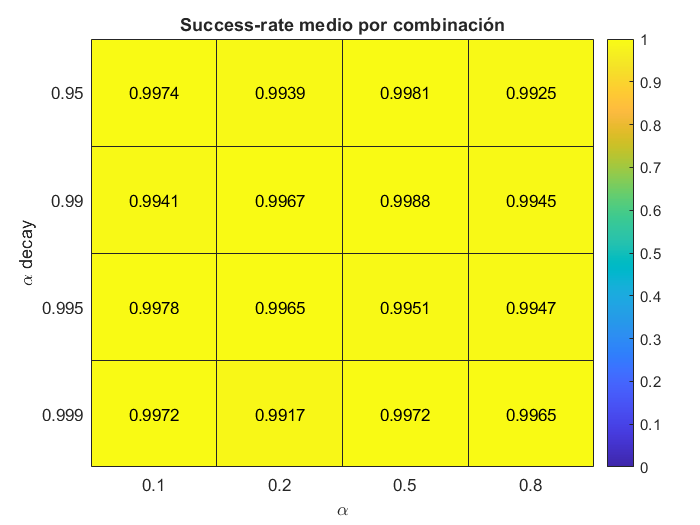
\includegraphics[width=0.7\textwidth]{../../experiments/qlearning/experiment-3/results/success.png}
    \caption{Tasa de éxito para diferentes combinaciones de $\alpha$ y su decaimiento}
    \label{fig:qlearning-success}
\end{figure}
La tasa de éxito también es muy elevada en este caso y no se observa ninguna tendencia clara. Todos los valores se encuentran entre el 99.17\% y el 99.88\%. 

A pesar de la poca diferencia, la mejor combinación se alcanza con $\alpha = 0.5$ y su decaimiento = 0.99, logrando una tasa de éxito del 99.88\%.


\newpage

\textbf{Recompensa media y número de pasos medios}

\begin{figure}[H]
    \centering
    \begin{subfigure}{0.7\textwidth}
        \centering
        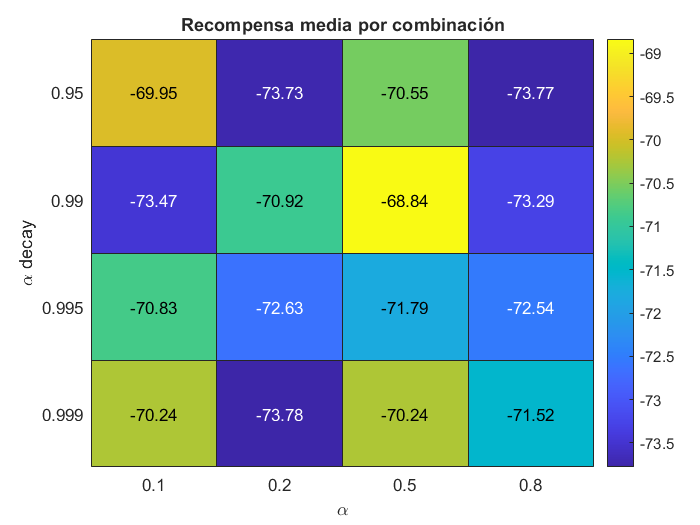
\includegraphics[width=\textwidth]{../../experiments/qlearning/experiment-3/results/reward.png}
        \caption{Recompensa media para diferentes combinaciones de $\alpha$ y su decaimiento}
        \label{fig:qlearning-subfig-reward}
    \end{subfigure}
    \hfill
    \begin{subfigure}{0.7\textwidth}
        \centering
        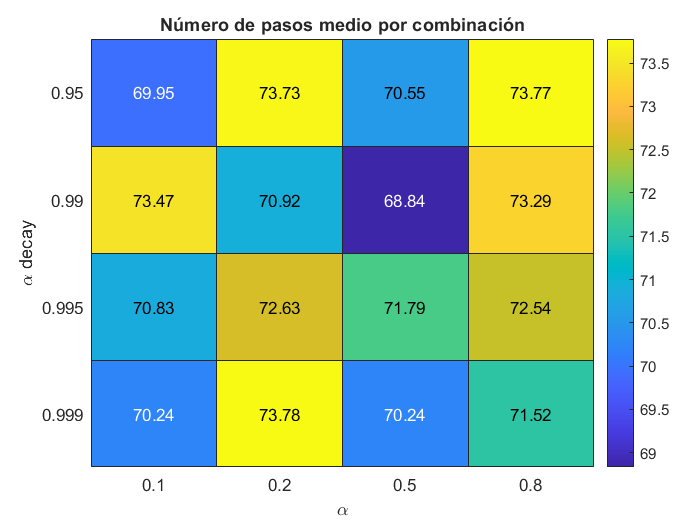
\includegraphics[width=\textwidth]{../../experiments/qlearning/experiment-3/results/steps.png}
        \caption{Número de pasos para diferentes combinaciones de $\alpha$ y su decaimiento}
        \label{fig:qlearning-subfig-steps}
    \end{subfigure}
    \caption{Análisis de la recompensa media y número de pasos}
    \label{fig:qlearning-reward}
\end{figure}

El análisis de la recompensa media y el número medio de pasos tampoco revela una tendencia clara. Lo que si que se puede observar es que todas las configuraciones se encuentran entre -73.78 y -68.84 de recompensa, lo que indica que ninguna de ellas se desvia ni obtiene resultados muy negativos. 
\\

Se puede observar también que el número medio de pasos corresponde exactamente con la recompensa media en cada configuración. Esto nos indica que el agente no cae por el barranco en ningún momento, ya que sino la recompensa media sería más negativa.
\\

Las combinación óptima es $\alpha = 0.5$ y su decaimiento = 0.99, logrando una recompensa media de -68.84.
\\

\textbf{Tiempo de entrenamiento}
\\

Para el tiempo de entrenamiento, se han elegido las tres combinaciones que mejor rendimiento han dado. 

\begin{figure}[H]
    \centering
    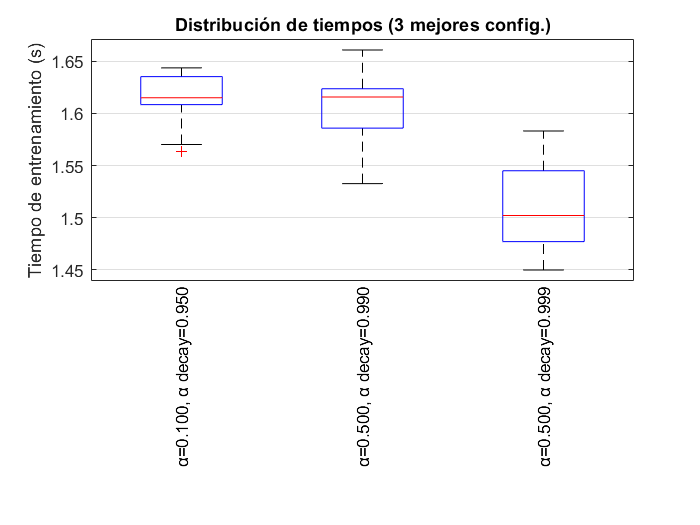
\includegraphics[width=0.8\textwidth]{../../experiments/qlearning/experiment-3/results/time.png}
    \caption{Tiempo de entrenamiento para diferentes combinaciones de $\alpha$ y su decaimiento}
    \label{fig:qlearning-time}
\end{figure}

En este caso se puede observar como una de las combinaciones tiene un tiempo de entrenamiento más bajo, concretamente la que tiene un decaimiento más lento. Esto puede ser debdido a que \alpha disminuye más lentamente y por lo tanto el algoritmo converge más rápido. Aún así, el tiempo de entrenamiento varia en pocas decimas de segundo.
\\

\newpage
\textbf{Tabla resumen}

\begin{table}[H]
    \centering
    \begin{tabular}{|c|c|l|r|c|}
    \hline
    $\alpha$ & $decay$ & Métrica        & Media    & Intervalo de Confianza del 95\% \\
    \hline
    0.10 & 0.95 & Success-rate  & 0.997   & [0.995, 1.000] \\
         &      & Rew. media    & -69.945 & [-72.926, -66.964] \\
         &      & Steps medios  & 69.9    & [67.0, 72.9] \\
         &      & Time (s)      & 1.62    & [1.60, 1.63] \\
    \hline
    0.50 & 0.99 & Success-rate  & 0.999   & [0.997, 1.000] \\
         &      & Rew. media    & -68.836 & [-71.366, -66.305] \\
         &      & Steps medios  & 68.8    & [66.3, 71.4] \\
         &      & Time (s)      & 1.61    & [1.58, 1.63] \\
    \hline
    0.50 & 0.999 & Success-rate  & 0.997   & [0.995, 1.000] \\
         &       & Rew. media    & -70.240 & [-73.155, -67.326] \\
         &       & Steps medios  & 70.2    & [67.3, 73.2] \\
         &       & Time (s)      & 1.51    & [1.48, 1.54] \\
    \hline
    \end{tabular}
    \caption{Resultados para combinaciones seleccionadas de $\alpha$ y $decay$}
    \label{tab:resultados_seleccionados}
\end{table}

    
\textbf{Conclusiones}
\\

Del análisis experimental se pueden extraer las siguientes conclusiones:

\begin{enumerate}
    \item La tasa de aprendizaje refinada y su decaimiento no parecen tener un impacto significativo en el rendimiento del algoritmo Q-Learning.
    \item La mejor combinación general considerando todas los métricas es $\alpha = \textbf{0.5}$ y su decaimiento = \textbf{0.99}, que proporciona:
    \begin{itemize}
        \item Una tasa de éxito del 99.88\%.
        \item Una recompensa media de -68.84.
        \item Un tiempo de entrenamiento de 1.61 segundos.
    \end{itemize}
    \item Los resultados obtenidos difieren ligeramente de la hipótesis inicial, ya que ha dado mejor resultado una tasa de aprendizaje moderada con un decaimiento lento. 
\end{enumerate}

Aunque los parámetros seleccionados no minimizan el tiempo de entrenamiento, las diferencias temporales observadas son mínimas. En este estudio se ha priorizado la optimización de la tasa de aciertos y la recompensa sobre el tiempo de entrenamiento, ya que estos criterios son más relevantes para evaluar la efectividad del algoritmo.

\subsubsection{Experimento número de episodios}

\paragraph{Diseño experimental}
El objetivo de este experimento es analizar cómo el número de episodios de entrenamiento afectan el rendimiento del algoritmo Q-Learning.
\begin{table}[H]
    \centering
    \begin{tabularx}{\textwidth}{|p{4cm}|X|} % Especificar el ancho de las columnas
        \hline % Línea horizontal superior
        \textbf{Observación} & El número de episodios de entrenamiento es un parámetro crítico en el algoritmo Q-Learning.
        \\ \hline
        \textbf{Planteamiento} & Se compara la tasa de acierto (llegar al estado final), la recompensa media, número de pasos y tiempo de entrenamiento del algoritmo para diferentes números de episodios de entrenamiento.
        \\ \hline
        \textbf{Hipótesis} & Un mayor número de episodios de entrenamiento mejorará el rendimiento del algoritmo.
        \\ \hline
        \textbf{Método} &
        \begin{itemize}
            \item Se fijan los mejores valores para \(\gamma\), \(\alpha\), decaimiento de \(\alpha\), \(\epsilon\), decaimiento de \(\epsilon\) de los experimentos anteriores y una penalización de la acción ``moverse a la izquierda'' de $-1$.
            \item Se eligen los siguientes \textit{números de episodios de entrenamiento}: \{500, 1000, 5000, 10000\}.
            \item Para cada \textit{número de episodios}, se ejecuta el algoritmo Q-Learning en el entorno.
            \item Se evalúa la política obtenida probándola con 500 episodios.
            \item Se repite el proceso para cada número de episodios 20 veces para obtener una muestra maś representativa (debido a la estocasticidad del entorno).
        \end{itemize}
        \\ \hline
    \end{tabularx}
    \caption{Q-Learning - Experimento 4 - Número de episodios}
    \label{tab:diseñoQLEarningExp3}
\end{table}


\paragraph{Resultados}

En este experimento, los resultados se han representado mediante boxplots ya que solo se está variando un parámetro. 
\\

\newpage
\textbf{Tasa de Éxito}

\begin{figure}[H]
    \centering
    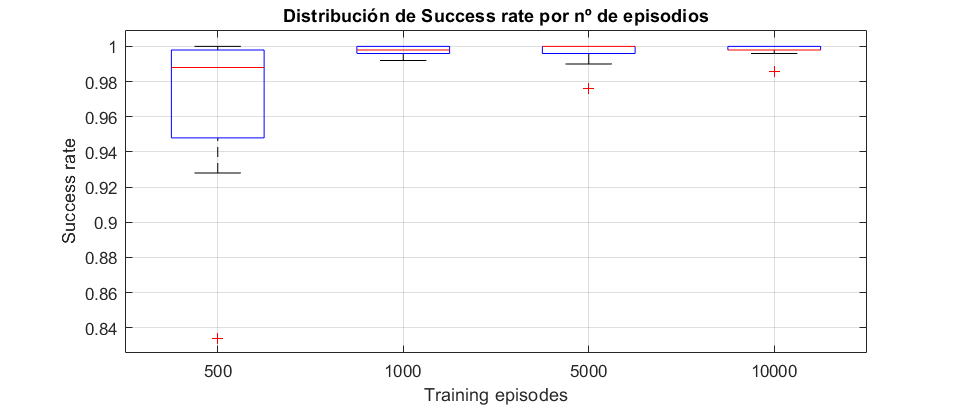
\includegraphics[width=0.9\textwidth]{../../experiments/qlearning/experiment-4/results/success.png}
    \caption{Tasa de éxito para diferentes números de episodios de entrenamiento}
    \label{fig:qlearning-success}
\end{figure}

 Se puede observar una ligera tendencia a mejorar la tasa de éxito al aumentar el número de episodios de entrenamiento. Además, se observa que la variabilidad de los valores también disminuye al aumentar el número de episodios.
\\

Según estos resultados, el mejor número de episodios de entrenamiento es 10000, con una tasa media de éxito del 99.87\%.
\\

\newpage
\textbf{Recompensa media y número de pasos medios}


\begin{figure}[H]
    \centering
    \begin{subfigure}{0.9\textwidth}
        \centering
        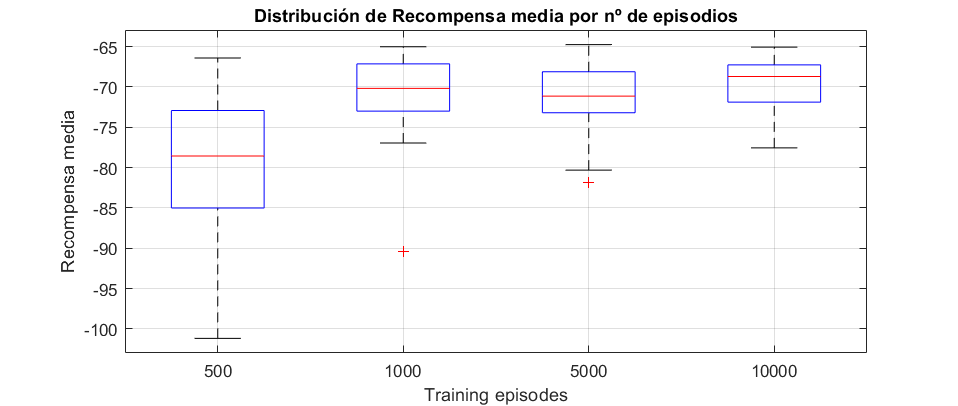
\includegraphics[width=\textwidth]{../../experiments/qlearning/experiment-4/results/reward.png}
        \caption{Recompensa media para diferentes números de episodios de entrenamiento}
        \label{fig:qlearning-subfig-reward}
    \end{subfigure}
    \hfill
    \begin{subfigure}{0.9\textwidth}
        \centering
        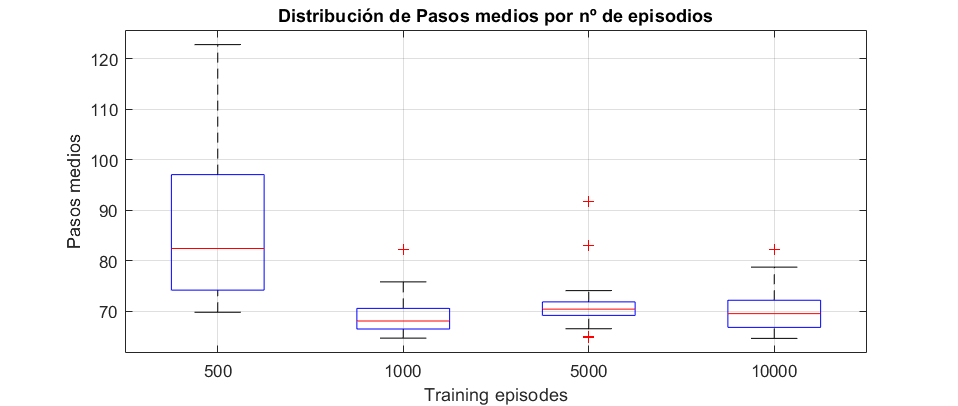
\includegraphics[width=\textwidth]{../../experiments/qlearning/experiment-4/results/steps.png}
        \caption{Número de pasos para diferentes números de episodios de entrenamiento}
        \label{fig:qlearning-subfig-steps}
    \end{subfigure}
    \caption{Análisis de la recompensa media y número de pasos}
    \label{fig:qlearning-reward}
\end{figure}

Con estos resultados se observa la misma tendencia que en la tasa de éxito. La recompensa media mejora conforme aumentan los episodios de entrenamiento y el número de pasos disminuyen. También se observa el "salto" significativo de 500 a 1000 episodios de entrenamiento, donde los resultados mejora notablemente. A partir de 1000 episodios, la mejora es más gradual. 
\\

\newpage

\textbf{Tiempo de entrenamiento}

\begin{figure}[H]
    \centering
    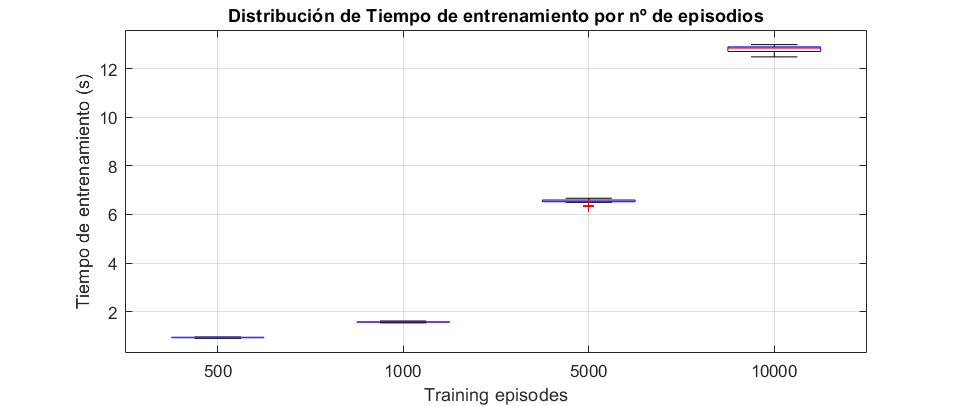
\includegraphics[width=0.9\textwidth]{../../experiments/qlearning/experiment-4/results/time.png}
    \caption{Tiempo de entrenamiento para diferentes números de episodios de entrenamiento}
    \label{fig:qlearning-time}
\end{figure}

Como es lógico, el tiempo de entrenamiento aumenta conforme aumentan los episodios de entrenamiento. El más costoso es el de 10000 episodios, con un tiempo medio de 12.8 segundos, el doble que el de 5000 (6.54 segundos).
\\

\textbf{Tabla resumen}

\begin{table}[h!]
    \centering
    \begin{tabular}{|c|l|r|c|}
    \hline
    Episodios & Métrica        & Media    & Intervalo de Confianza del 95\% \\
    \hline
    500   & Success-rate  & 0.988   & [0.984, 0.992] \\
          & Rew. media    & -79.584 & [-82.496, -76.671] \\
          & Pasos medios  & 79.6    & [76.7, 82.5] \\
          & Tiempo (s)    & 0.93    & [0.93, 0.94] \\
    \hline
    1000  & Success-rate  & 0.996   & [0.993, 0.998] \\
          & Rew. media    & -71.112 & [-72.871, -69.354] \\
          & Pasos medios  & 71.1    & [69.4, 72.9] \\
          & Tiempo (s)    & 1.58    & [1.57, 1.59] \\
    \hline
    5000  & Success-rate  & 0.996   & [0.994, 0.998] \\
          & Rew. media    & -71.358 & [-72.781, -69.934] \\
          & Pasos medios  & 71.4    & [69.9, 72.8] \\
          & Tiempo (s)    & 6.54    & [6.52, 6.57] \\
    \hline
    10000 & Success-rate  & 0.998   & [0.997, 0.999] \\
          & Rew. media    & -69.626 & [-70.662, -68.591] \\
          & Pasos medios  & 69.6    & [68.6, 70.7] \\
          & Tiempo (s)    & 12.80   & [12.75, 12.84] \\
    \hline
    \end{tabular}
    \caption{Resultados del algoritmo cantidades de episodios de entrenamiento}
    \label{tab:qlearning_episodios}
\end{table}
    

\textbf{Conclusiones}
\\

Del análisis experimental se pueden extraer las siguientes conclusiones:

\begin{enumerate}
    \item El número de episodios de entrenamiento afecta considerablemente al rendimiento del algoritmo.
    \item El número de episodios de entrenamiento afecta considerablemente al tiempo de entrenamiento.
    \item El número de episodios con mejor trade off entre rendimiento y tiempo de entrenamiento es \textbf{5000}, que proporciona:
    \begin{itemize}
        \item Una tasa de éxito del 99.6\%.
        \item Una recompensa media de -71.112.
        \item Un tiempo de entrenamiento de 6.54 segundos.
    \end{itemize}
    \item Los resultados obtenidos confirman la hipótesis inicial de que un mayor número de episodios de entrenamiento mejora el rendimiento del algoritmo.
\end{enumerate}

\newpage
\subsubsection{Experimento penalización de la acción izquierda}

\paragraph{Diseño experimental}
El objetivo de este experimento es analizar si penalizar acciones poco favorables afectan el rendimiento del algoritmo Q-Learning.
\begin{table}[H]
    \centering
    \begin{tabularx}{\textwidth}{|p{4cm}|X|} % Especificar el ancho de las columnas
        \hline % Línea horizontal superior
        \textbf{Observación} & Moverse a la izquierda no es deseable para el agente en ningún momento, ya que no le acerca al objetivo. Por lo tanto, penalizarla con una recompensa menor que las demás acciones puede alterar el comportamiento del agente.
        \\ \hline 
        \textbf{Planteamiento} & Se compara la tasa de acierto (llegar al estado final), la recompensa media, número de pasos y tiempo de entrenamiento del algoritmo para diferentes penalizaciones a la acción ``moverse a la izquierda''.
        \\ \hline
        \textbf{Hipótesis} & Penalizar la acción ``moverse a la izquierda'' mejorará el rendimiento del algoritmo.
        \\ \hline
        \textbf{Método} &
        \begin{itemize}
            \item Se fijan los mejores valores para \(\gamma\), \(\alpha\), decaimiento de \(\alpha\), \(\epsilon\), decaimiento de \(\epsilon\) de los experimentos anteriores.
            \item Se eligen los siguientes valores para la penalización de la acción ``moverse a la izquierda'': \{-1, -2, -10, -50\}.
            \item Para cada penalización, se ejecuta el algoritmo Q-Learning en el entorno.
            \item Se evalúa la política obtenida probándola con 500 episodios.
            \item Se repite el proceso para cada penalización 20 veces para obtener una muestra más significativa (debido a la estocasticidad del entorno).
        \end{itemize}
        \\ \hline
    \end{tabularx}
    \caption{Q-Learning - Experimento 5 - Penalización de la acción ``moverse a la izquierda''}
    \label{tab:diseñoQLEarningExp4}
\end{table}

\paragraph{Resultados}
En este experimento, los resultados se han representado mediante boxplots ya que solo se está variando un parámetro. 
\\

\newpage
\textbf{Tasa de Éxito}

\begin{figure}[H]
    \centering
    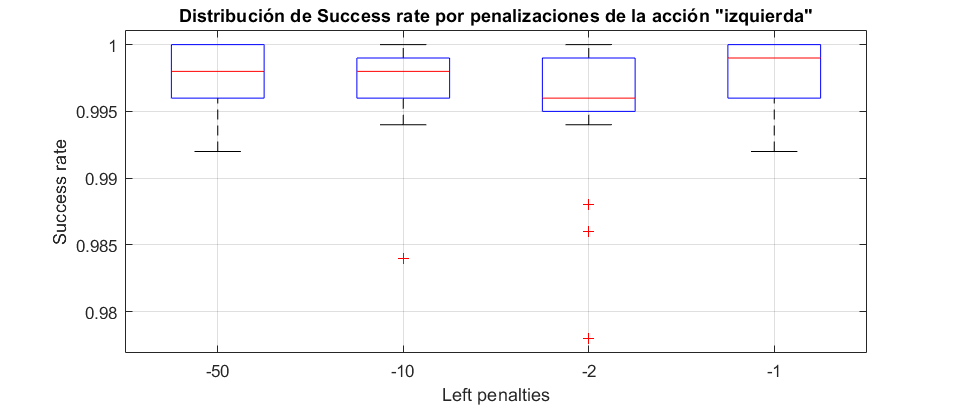
\includegraphics[width=0.8\textwidth]{../../experiments/qlearning/experiment-5/results/success.png}
    \caption{Tasa de éxito para diferentes valores de penalización a la acción ``moverse a la izquierda''}
    \label{fig:qlearning-success}
\end{figure}

No se aprecia una gran diferencia en cuanto a la tasa de éxito. Todas las medias se encuentran por encima del 99\% y la variabilidad es muy baja. 
\\

\newpage
\textbf{Recompensa media y número de pasos medios}


\begin{figure}[H]
    \centering
    \begin{subfigure}{0.7\textwidth}
        \centering
        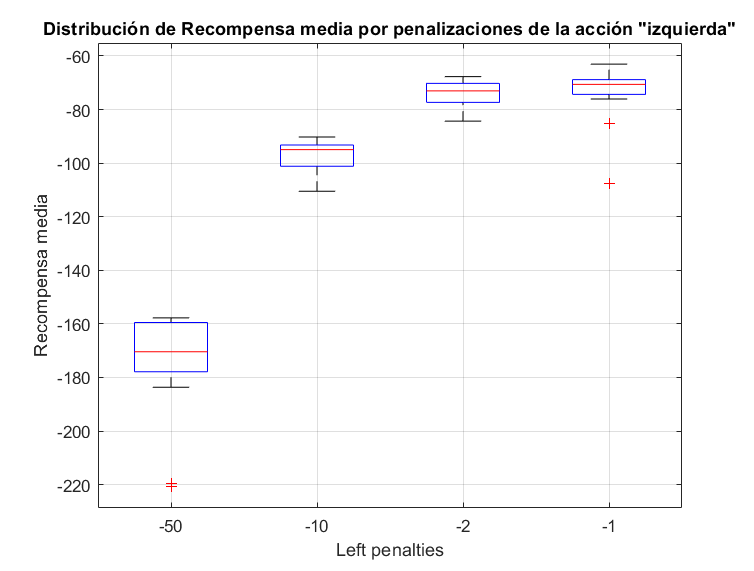
\includegraphics[width=\textwidth]{../../experiments/qlearning/experiment-5/results/reward.png}
        \caption{Recompensa media para diferentes valores de penalización a la acción ``moverse a la izquierda''}
        \label{fig:qlearning-subfig-reward}
    \end{subfigure}
    \hfill
    \begin{subfigure}{0.7\textwidth}
        \centering
        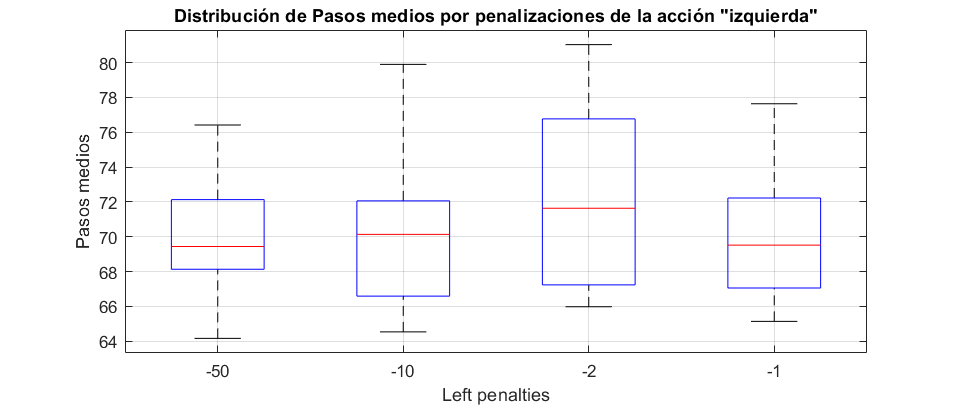
\includegraphics[width=\textwidth]{../../experiments/qlearning/experiment-5/results/steps.png}
        \caption{Número de pasos para diferentes valores de penalización a la acción ``moverse a la izquierda''}
        \label{fig:qlearning-subfig-steps}
    \end{subfigure}
    \caption{Análisis de la recompensa media y número de pasos}
    \label{fig:qlearning-reward}
\end{figure}

Para seguir con la estructura de los experimentos anteriores, se muestran los boxplots de la recompensa media y el número de pasos medios. En este caso, del boxplot de la recompensa media no se puede deducir nada, ya que al haber modificado la penalización, cada recompensa media es relativa a la penalización. Sin embargo, se puede medir el rendimiento mediante el número de pasos medios. En este caso, se observa una muy ligera tendencia a mejorar el rendimiento al aumentar la penalización. 
\\

\textbf{Tiempo de entrenamiento}

\begin{figure}[H]
    \centering
    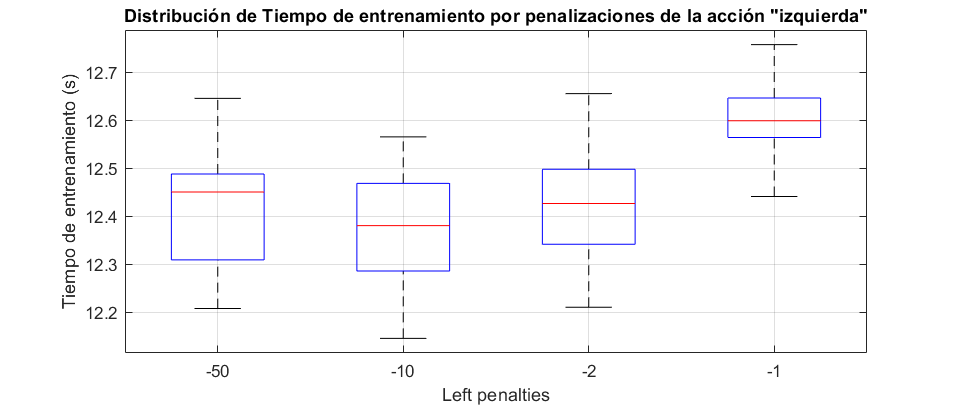
\includegraphics[width=0.8\textwidth]{../../experiments/qlearning/experiment-5/results/time.png}
    \caption{Tiempo de entrenamiento para diferentes valores de penalización a la acción ``moverse a la izquierda''}
    \label{fig:qlearning-time}
\end{figure}

El tiempo de se un poco reducido con penalizaciones más altas que 1, pero no se observa una tendencia clara. 
\\

\newpage
\textbf{Tabla resumen}

\begin{table}[H]
    \centering
    \begin{tabular}{|c|l|r|c|}
    \hline
    Left penalty & Métrica        & Media    & Intervalo de Confianza del 95\% \\
    \hline
    -50  & Success-rate  & 0.998     & [0.998, 0.999] \\
         & Rew. media    & -173.343  & [-179.002, -167.685] \\
         & Pasos medios  & 69.4      & [68.4, 70.3] \\
         & Tiempo (s)    & 12.56     & [12.51, 12.61] \\
    \hline
    -10  & Success-rate  & 0.997     & [0.995, 0.998] \\
         & Rew. media    & -97.021   & [-98.710, -95.332] \\
         & Pasos medios  & 69.8      & [68.2, 71.3] \\
         & Tiempo (s)    & 12.46     & [12.43, 12.50] \\
    \hline
    -2   & Success-rate  & 0.997     & [0.996, 0.998] \\
         & Rew. media    & -74.077   & [-75.488, -72.666] \\
         & Pasos medios  & 71.0      & [69.6, 72.5] \\
         & Tiempo (s)    & 12.48     & [12.44, 12.53] \\
    \hline
    -1   & Success-rate  & 0.992     & [0.986, 0.998] \\
         & Rew. media    & -73.278   & [-76.204, -70.352] \\
         & Pasos medios  & 73.3      & [70.4, 76.2] \\
         & Tiempo (s)    & 12.74     & [12.71, 12.78] \\
    \hline
    \end{tabular}
    \caption{Resultados del algoritmo para diferentes valores de penalización por ir a la izquierda}
    \label{tab:qlearning_penalizaciones}
    \end{table}
    

\textbf{Conclusiones}
\\

Del análisis experimental se pueden extraer las siguientes conclusiones:

\begin{enumerate}
    \item La penalización de la acción ``moverse a la izquierda'' no parece tener un impacto significativo en el rendimiento del algoritmo.
    \item El mejor valor de penalización obtenido es \textbf{-50}, que proporciona:
    \begin{itemize}
        \item Una tasa de éxito del 99.8\%.
        \item Un número medio de pasos de 69.4.
        \item Un tiempo de entrenamiento de 12.56 segundos.
    \end{itemize}
    \item Los resultados obtenidos difieren ligeramente de la hipótesis inicial, ya que no se observa una mejora muy significativa al penalizar la acción ``moverse a la izquierda''.
\end{enumerate}